\documentclass[11pt]{article}
\usepackage{euscript}

\usepackage{amsmath,amssymb,bm}
\usepackage{amsthm}
\usepackage{amssymb}
\usepackage{epsfig}
\usepackage{xspace}
\usepackage{color}
\usepackage{url}
\usepackage{subfigure}
\usepackage{enumerate}

%%%%%%%  For drawing trees  %%%%%%%%%
\usepackage{tikz}
\usetikzlibrary{calc, shapes, backgrounds}

%%%%%%%%%%%%%%%%%%%%%%%%%%%%%%%%%
\setlength{\textheight}{9in}
\setlength{\topmargin}{-0.600in}
\setlength{\headheight}{0.2in}
\setlength{\headsep}{0.250in}
\setlength{\footskip}{0.5in}
\flushbottom
\setlength{\textwidth}{6.5in}
\setlength{\oddsidemargin}{0in}
\setlength{\evensidemargin}{0in}
\setlength{\columnsep}{2pc}
\setlength{\parindent}{0em}
%%%%%%%%%%%%%%%%%%%%%%%%%%%%%%%%%


\newcommand{\eps}{\varepsilon}

\renewcommand{\c}[1]{\ensuremath{\EuScript{#1}}}
\renewcommand{\b}[1]{\ensuremath{\mathbb{#1}}}
\newcommand{\s}[1]{\textsf{#1}}

\newcommand{\E}{\textbf{\textsf{E}}}
\renewcommand{\Pr}{\textbf{\textsf{Pr}}}

\title{Data Visualization Course Project Proposal}
\author{Zhuoyue Zhao, Ya Gao\\\{zyzhao, ygao\}@cs.utah.edu}
\date{}

\begin{document}
\maketitle

\paragraph{Basic Info.} Visualization for FDIC Failed Bank List

Group members:

Zhuoyue Zhao (u1065756), zyzhao@cs.utah.edu

Ya Gao (u1137971), ygao@cs.utah.edu

https://github.com/zzy7896321/dataviscourse-pr-fdicfailedbanks


\paragraph{Background and Motivation.}

We looked at the resources on the course web page and found this FDIC failed
bank list. FDIC (Federal Deposit Insurance Corporation) was created in 1933
to restore public confidence in banking during the Greate Depression in the
1930s.  It insures a depositor for up to \$250,000 in a FDIC member bank in
the event of a bank failure. FDIC usually find a bank that is willing to
acquire a failed bank so that the deposits are simply transferred to the new
bank. However, sometimes, it cannot find a acquiring bank and will send the
insured funds directly to the customers. It is amazing that no depositor has
ever lost FDIC insured funds since its establishment but it is also worrying
that a massive wave of bank failures or a large bank failure could fail FDIC.
We are curious about how reliable FDIC has been and will be in the future.

\paragraph{Project Objectives.} 
We plan to visualize the spatio-temporal FDIC bank failures as well as the
distribution of acquiring banks. 1) The primary goal is to get an idea about
how useful and reliable FDIC has been in the past. 2) We might also want to
know how likely will FDIC fail if a lot of bank or a large bank fails based on
the peak period of failure in history. 3) We want to use d3 and svg to create
the visualization. We also want to use brushing and linking to allow exploring
the details of the data.

\paragraph{Data.}
We downloaded a detailed list of FDIC failed banks from 1934. It can be
obtained by launching the select-all query at
\url{https://www5.fdic.gov/hsob/SelectRpt.asp?EntryTyp=30&Header=1}. It
includes the name, the location of the headquarter, the effective date, the
total deposits, the total assets and other data of the banks.

We also have a second list of FDIC failed banks from October 1, 2000, available
at \url{https://www.fdic.gov/bank/individual/failed/banklist.html}. In
addition to the data available in the first table, it also lists the acquiring
institutions of the failed banks.

\paragraph{Data Processing.}
The data in both tables are quite clean. There are a few missing values in
irrelevant columns and the estimated loss column. To deal with that, we'll
ignore those rows with missing values in the estimated loss column. There are
4095 records in the table, which might be too many for our purpose. We are
considering restricting the data to starting from October 1, 2000. We also
plan to do some aggregations over the data on the numeric columns grouped by
either year or state so that we can have a spatio-temporal summary of the
data. We can also compute the statistics of failed banks each acquiring
institutions acquired by joining the two table. That's the second reason why
we will restrict the data in the first table to the ones after October 1,
2000.

\paragraph{Visualization Design.} We proposed the following 3 prototype designs.

\begin{enumerate}[\textrm{Design} 1)]
    \item See Figure \ref{fig:design_1}.

        \begin{figure}[!h]
            \centering
            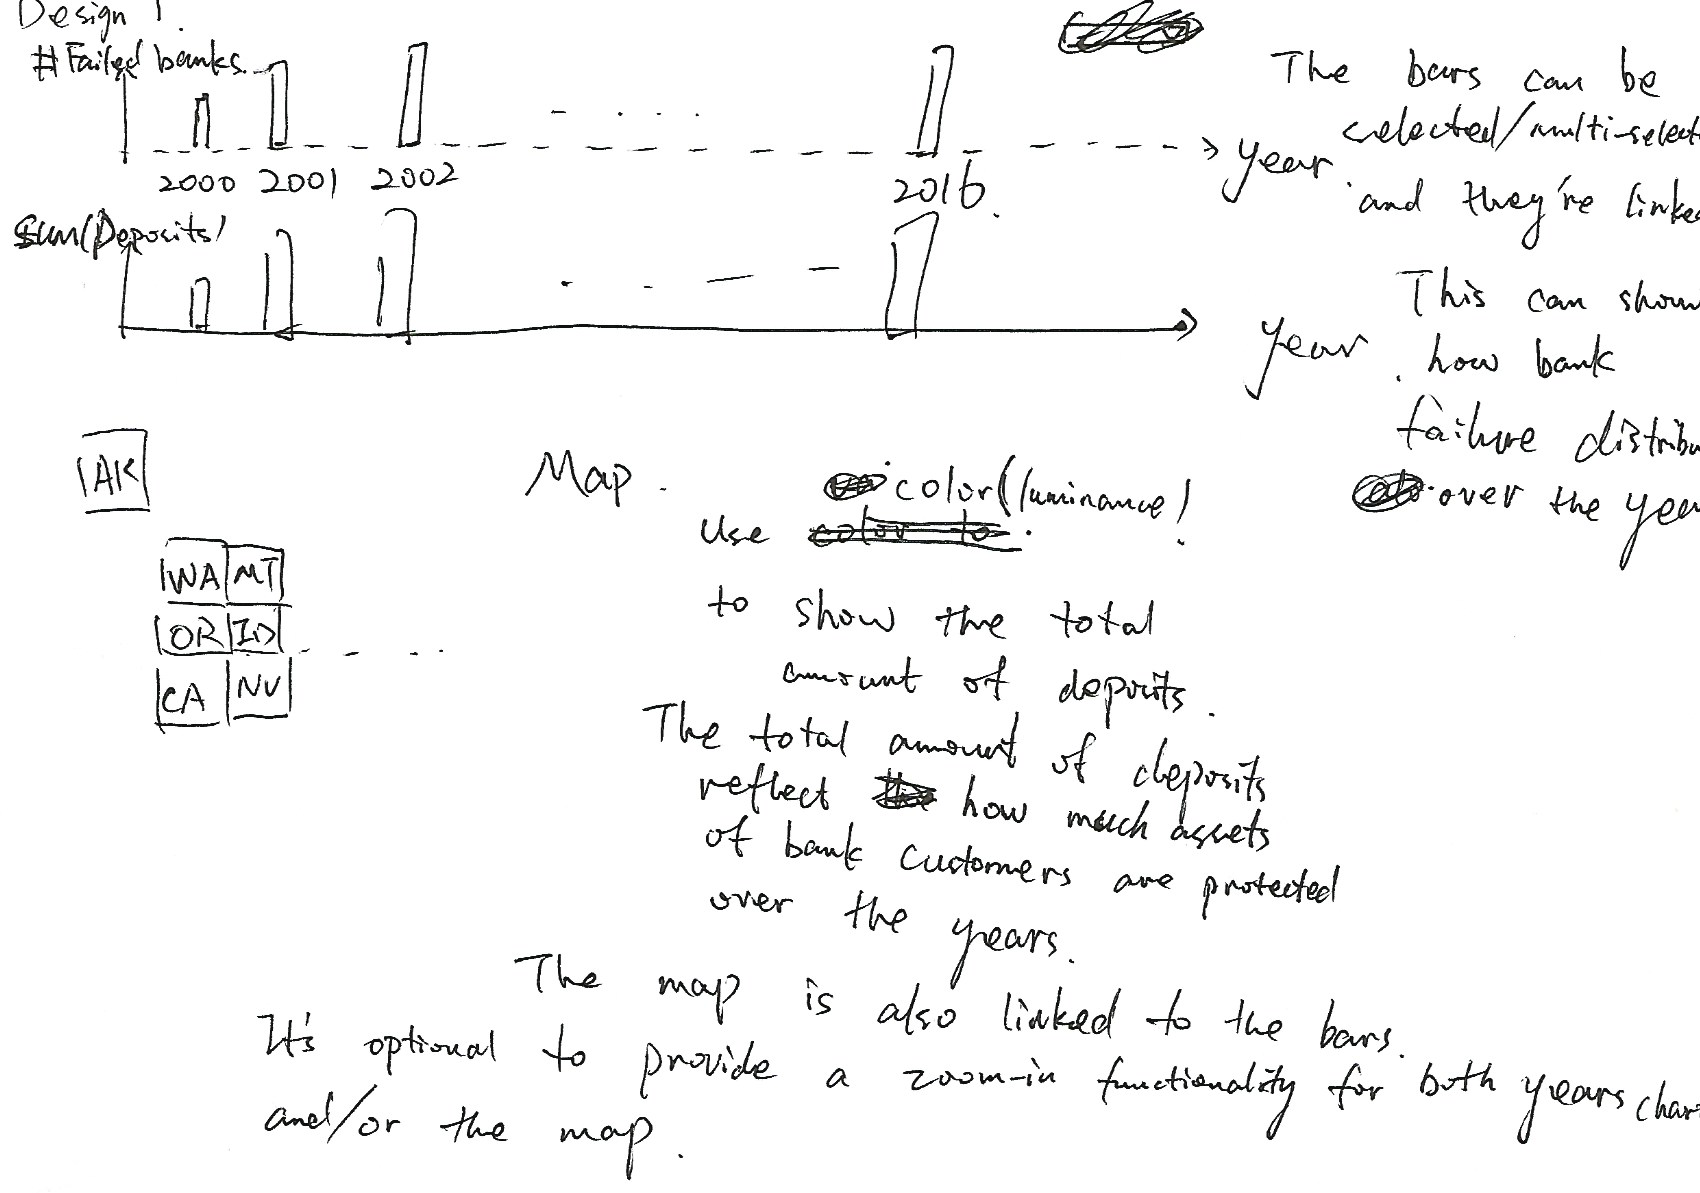
\includegraphics[width=0.9\textwidth]{fig/design_1}
            \caption{Design 1}
            \label{fig:design_1}
        \end{figure}

    \item See Figure \ref{fig:design_2}.

        \begin{figure}[!h]
            \centering
            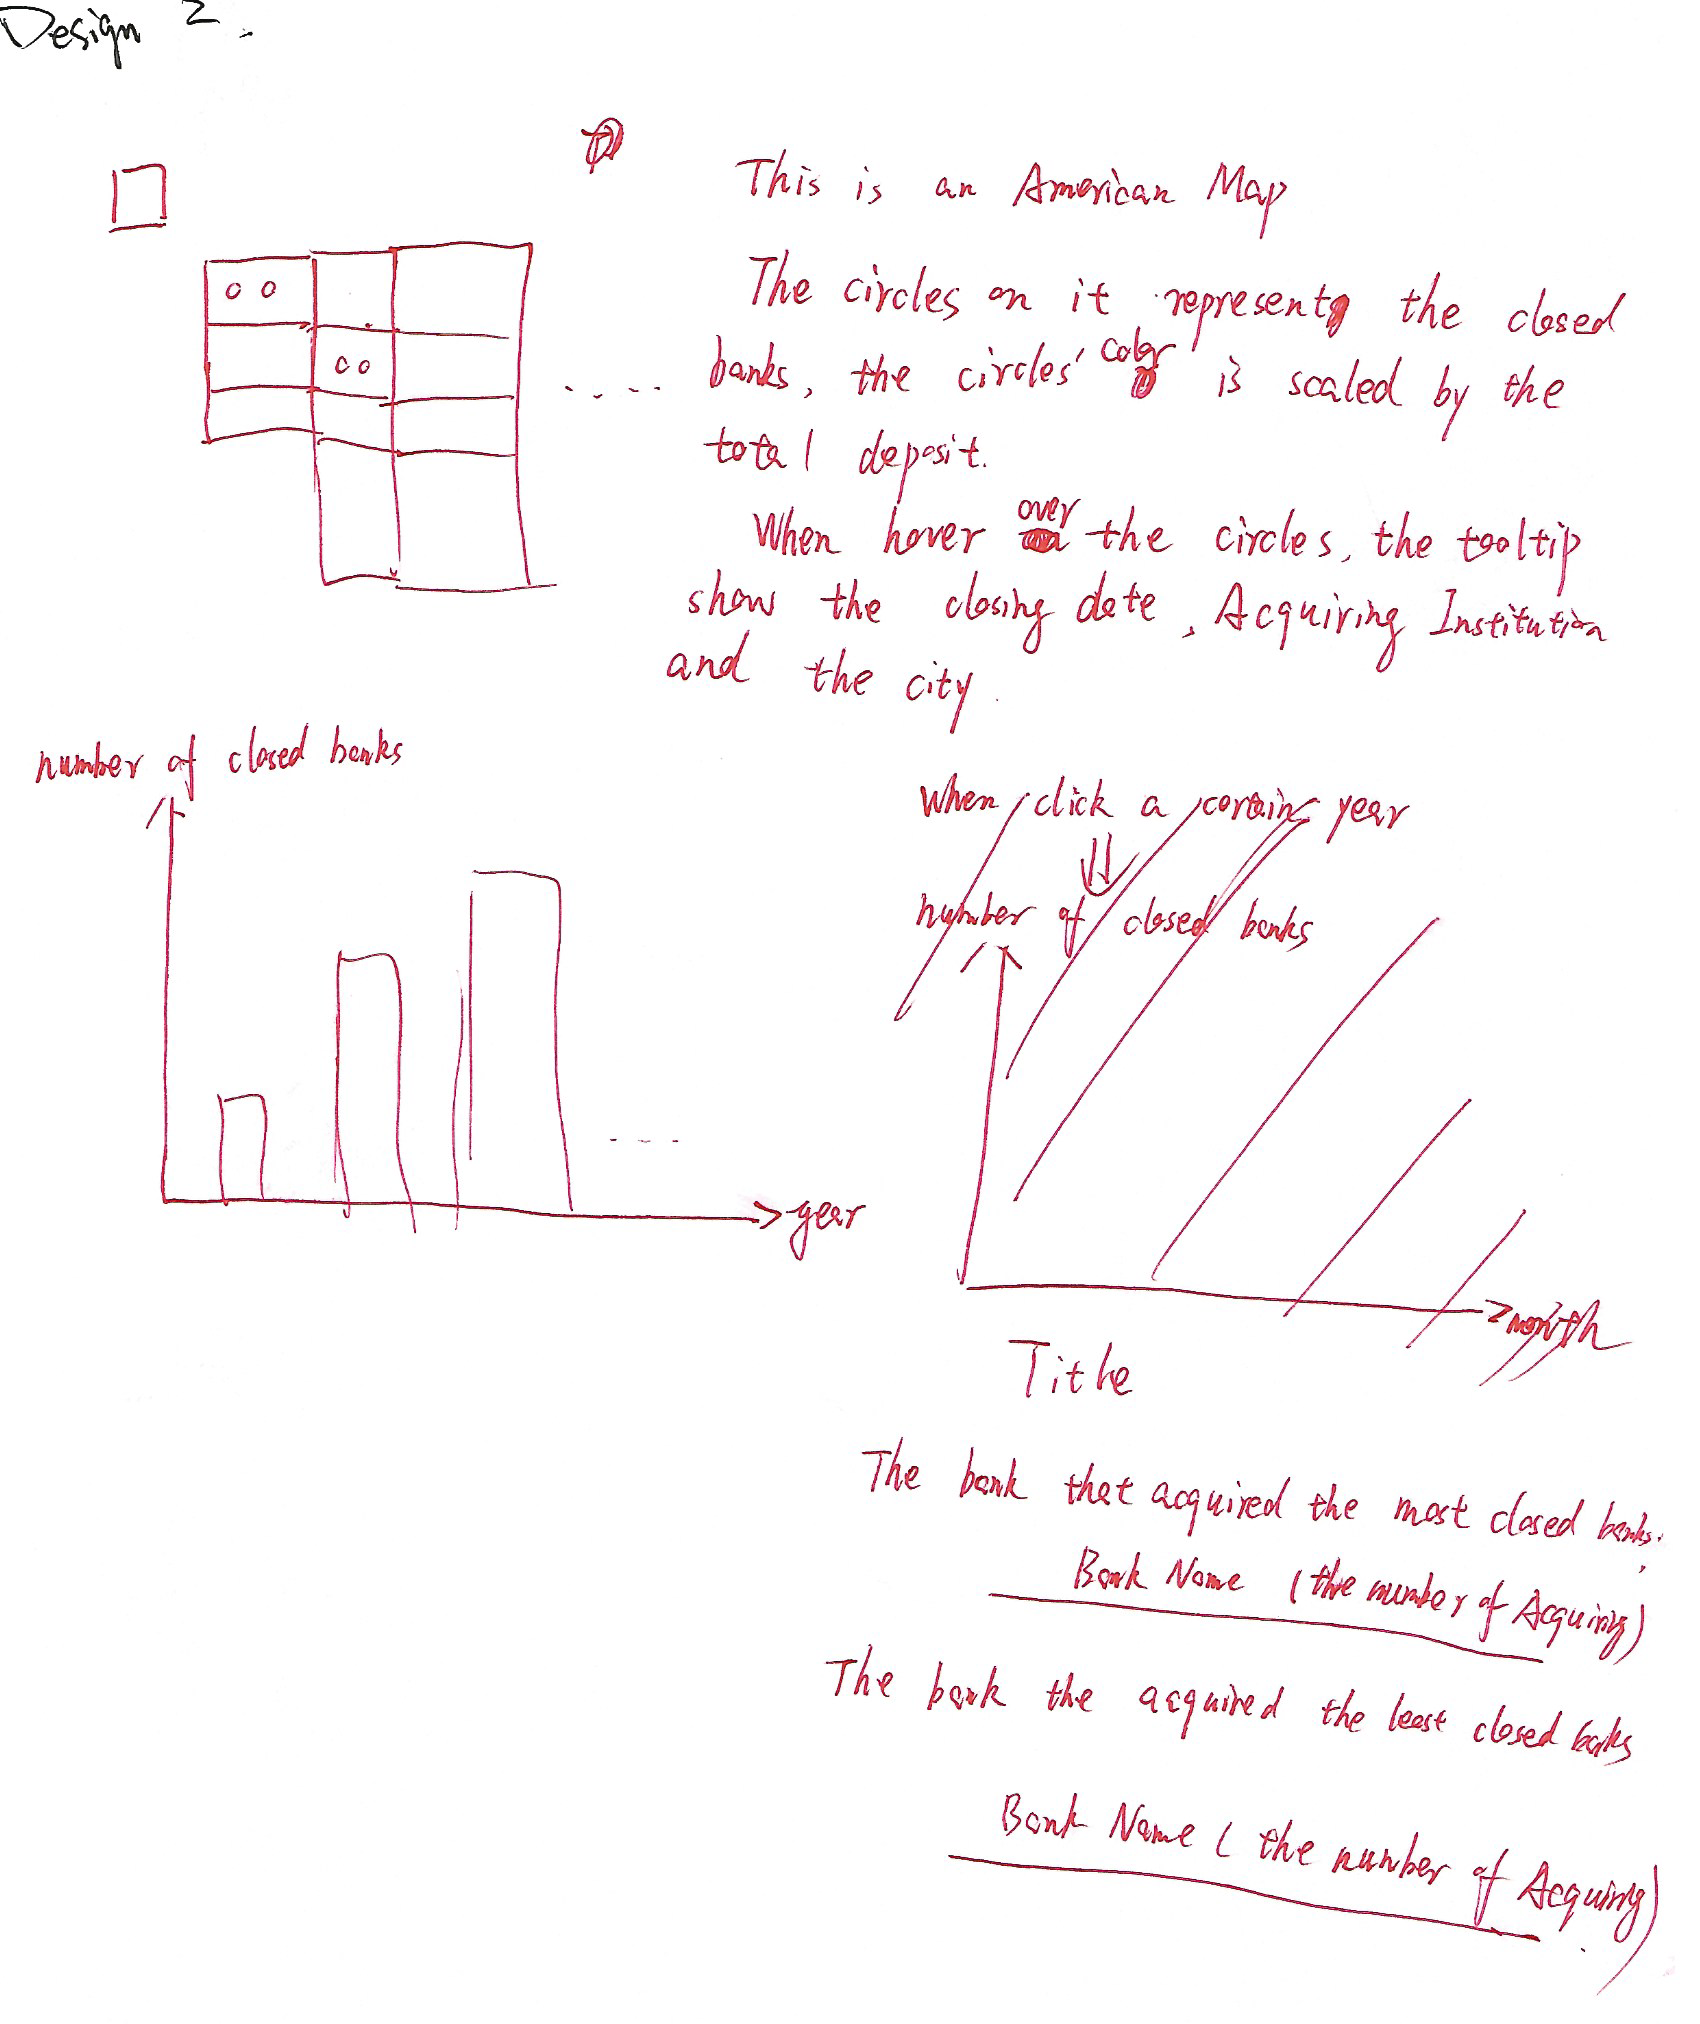
\includegraphics[width=0.9\textwidth]{fig/design_2}
            \caption{Design 2}
            \label{fig:design_2}
        \end{figure}

    \item See Figure \ref{fig:design_3}.
        
        \begin{figure}[!h]
            \centering
            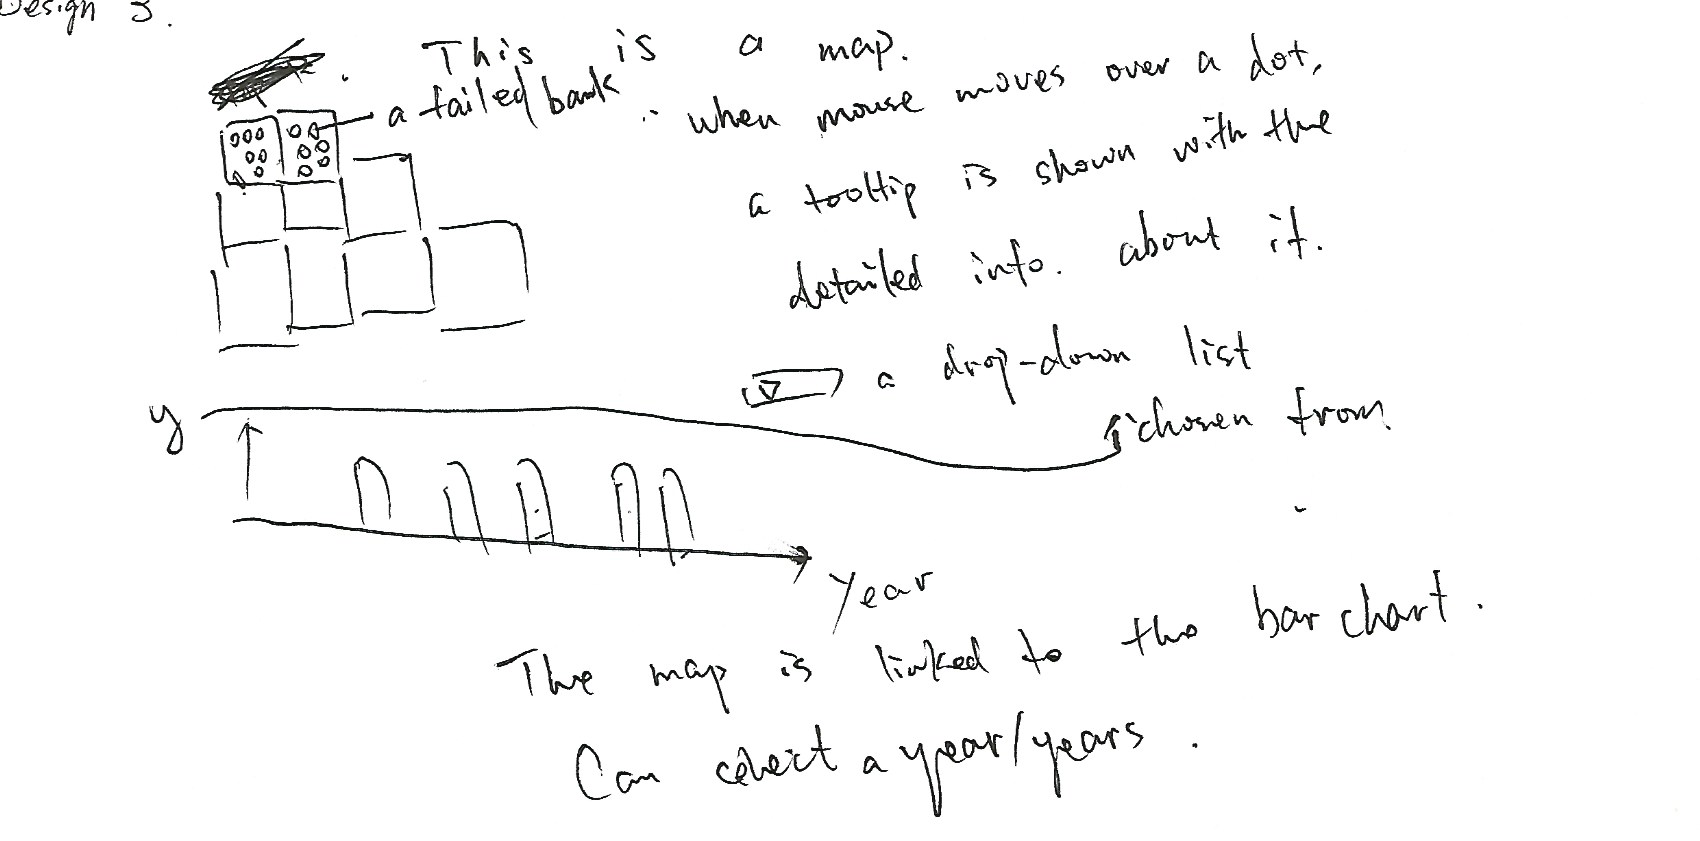
\includegraphics[width=0.9\textwidth]{fig/design_3}
            \caption{Design 3}
            \label{fig:design_3}
        \end{figure}
\end{enumerate}

After weighing the benefits and drawbacks of the ideas in each design, we
decided on the following final design (see Figure \ref{fig:final_design}).

\begin{figure}[!h]
    \centering
    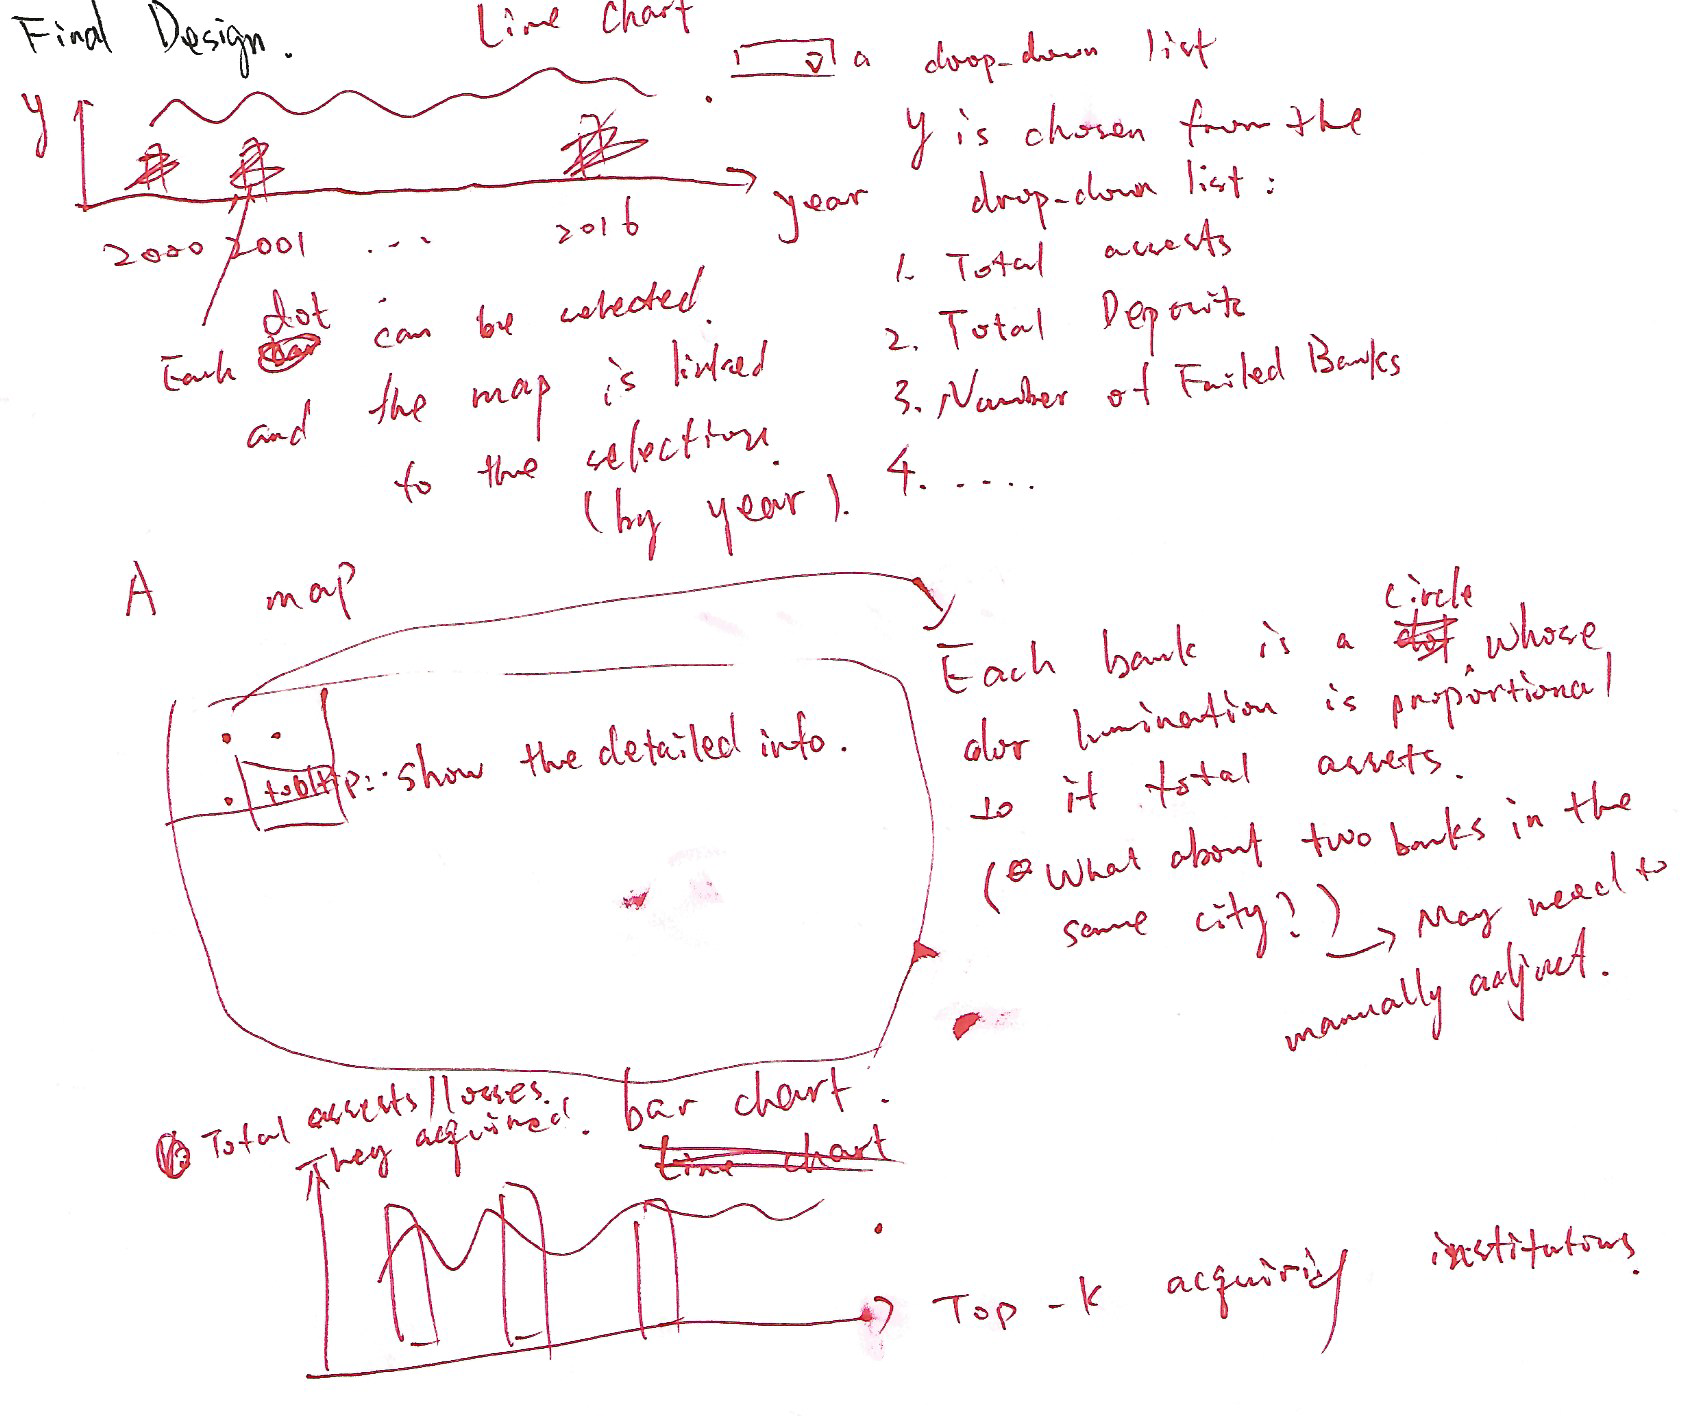
\includegraphics[width=0.9\textwidth]{fig/final_design}
    \caption{Final Design}
    \label{fig:final_design}
\end{figure}

\end{document}
